\section{Cơ sở lý thuyết}
\subsection{Mô hình Tối ưu hóa}

\hspace{0.5cm}
Mô hình tối ưu hóa là một phương pháp cơ bản trong toán học và khoa học máy tính nhằm tìm ra giải pháp tốt nhất trong số các phương án khả thi \cite{GiordanoFoxHorton}. Phương pháp này bao gồm việc xây dựng một mô hình toán học để tối đa hóa hoặc tối thiểu hóa một hàm mục tiêu cụ thể, đồng thời thỏa mãn một tập hợp các ràng buộc. Các mô hình tối ưu hóa được ứng dụng rộng rãi trong nhiều lĩnh vực như sản xuất, logistics và tài chính, nơi ra quyết định tối ưu đóng vai trò quan trọng trong việc cải thiện hiệu quả và giảm chi phí.

\subsubsection{Cấu trúc Cơ bản của Mô hình}
\hspace{0.5cm}Cấu trúc cơ bản của một mô hình tối ưu hóa như sau:
\[
\text{Tối ưu hóa } f_j(X) \quad \text{với } j \in J
\]
với các điều kiện ràng buộc:
\[
g_i(X) \{=, \leq, \geq\} b_i \quad \text{với mọi } i \in I
\]
Mục tiêu là tìm một vectơ \( X_0 \) sao cho tối ưu hóa các hàm mục tiêu \( f_j(X) \) với mọi \( j \in J \), đồng thời thỏa mãn các ràng buộc \( g_i(X) = b_i \) với mọi \( i \in I \).

\subsubsection{Giải thích Ký hiệu}
\hspace{0.5cm}Trong mô hình này:

- Thuật ngữ \textit{Tối ưu hóa} ám chỉ mục tiêu là tối đa hóa hoặc tối thiểu hóa hàm mục tiêu.

- Chỉ số \( j \) biểu thị rằng có thể có nhiều hàm mục tiêu, mỗi hàm tương ứng với một giá trị khác nhau của \( j \) trong tập hữu hạn \( J \).

- Vectơ \( X \) đại diện cho các biến quyết định, là các giá trị cần được xác định trong quá trình tối ưu hóa.

- Các hàm \( f_j(X) \) được gọi là hàm mục tiêu, chúng định nghĩa mục tiêu của bài toán tối ưu hóa.

- Thuật ngữ \textit{với các điều kiện ràng buộc} chỉ ra rằng các điều kiện, được gọi là ràng buộc, phải được thỏa mãn.

- Chỉ số \( i \) biểu thị các ràng buộc, trong đó mỗi hàm \( g_i(X) \) là một hàm ràng buộc mà vectơ nghiệm \( X_0 \) phải thỏa mãn. Các ràng buộc này có thể là phương trình hoặc bất phương trình, tùy thuộc vào bài toán.

- Các hằng số \( b_i \) đại diện cho giá trị ở phía phải của các ràng buộc, xác định giá trị cần thiết cho mỗi hàm ràng buộc \( g_i(X) \).

\subsubsection{Giải pháp cho Bài toán Tối ưu hóa}
\hspace{0.5cm}Giải pháp cho bài toán tối ưu hóa liên quan đến việc xác định vectơ \( X_0 \) sao cho tối ưu hóa mỗi hàm mục tiêu \( f_j(X) \), đồng thời thỏa mãn tất cả các ràng buộc \( g_i(X) = b_i \) \cite{GiordanoFoxHorton}. Tùy thuộc vào độ phức tạp của bài toán, có thể sử dụng nhiều phương pháp khác nhau như lập trình tuyến tính, lập trình nguyên, hoặc các thuật toán heuristic để tìm ra lời giải tối ưu.

\subsection{Lập trình Tuyến tính (Linear Programming - LP)}

\hspace{0.5cm}
Lập trình tuyến tính là một kỹ thuật tối ưu hóa toán học, trong đó mục tiêu là tối đa hóa hoặc tối thiểu hóa một hàm tuyến tính, đồng thời thỏa mãn một tập hợp các ràng buộc tuyến tính. Các biến quyết định trong bài toán lập trình tuyến tính được ký hiệu là \(x_j\) với \(j = 1, 2, \dots, n\), và hàm mục tiêu là một tổ hợp tuyến tính của các biến này. Cụ thể, hàm mục tiêu được biểu diễn như sau:

\[
\zeta = c_1 x_1 + c_2 x_2 + \cdots + c_n x_n
\]

trong đó \(c_1, c_2, \dots, c_n\) là các hằng số. Trong lập trình tuyến tính, mục tiêu thường là tối đa hóa hàm này, mặc dù các bài toán tối thiểu hóa cũng hợp lệ thông qua phép biến đổi đơn giản (tối đa hóa \(\zeta\) hoặc tối thiểu hóa \(-\zeta\)).

Bài toán lập trình tuyến tính có thể được mô tả như sau:

\begin{equation}
\text{Tối đa hóa } c_1 x_1 + c_2 x_2 + \dots + c_n x_n
\end{equation}
với các điều kiện ràng buộc:

\[
a_{11} x_1 + a_{12} x_2 + \dots + a_{1n} x_n \leq b_1
\]
\[
a_{21} x_1 + a_{22} x_2 + \dots + a_{2n} x_n \leq b_2
\]
\[
\vdots
\]
\[
a_{m1} x_1 + a_{m2} x_2 + \dots + a_{mn} x_n \leq b_m
\]

với điều kiện:

\[
x_1, x_2, \dots, x_n \geq 0
\]

trong đó \(m\) là số lượng ràng buộc, và \(n\) là số lượng biến quyết định.

Một \textit{nghiệm khả thi} là nghiệm thỏa mãn tất cả các ràng buộc, và một \textit{nghiệm tối ưu} là nghiệm tối đa hóa hoặc tối thiểu hóa hàm mục tiêu đồng thời thỏa mãn các ràng buộc.

Lập trình tuyến tính nguyên (ILP) là một biến thể của lập trình tuyến tính, trong đó các biến quyết định \(x_j\) được yêu cầu nhận giá trị nguyên. Bài toán ILP có thể được mô tả tương tự như bài toán LP nhưng thêm điều kiện rằng các biến \(x_j\) phải thuộc tập hợp các số nguyên.

Nới lỏng lập trình tuyến tính (LP Relaxation) là quá trình chuyển đổi một bài toán ILP thành bài toán LP bằng cách bỏ điều kiện ràng buộc các biến \(x_j\) phải là số nguyên. Điều này cho phép các biến \(x_j\) nhận các giá trị thực không âm, từ đó làm cho bài toán dễ giải hơn nhờ các thuật toán lập trình tuyến tính như phương pháp đơn hình (simplex method).

Nghiệm tối ưu của bài toán LP Relaxation là nghiệm tối ưu của ILP chỉ khi tất cả các biến trong nghiệm tối ưu của LP Relaxation đều nhận giá trị nguyên. Nếu không, cần áp dụng các kỹ thuật bổ sung để tìm nghiệm nguyên. Nghiệm của bài toán LP Relaxation sẽ được sử dụng làm cơ sở để tiếp tục giải bài toán ILP.


\subsection{Phương pháp Heuristic}

\hspace{0.5cm}Trong tối ưu hóa và giải quyết vấn đề, \textbf{heuristic} là các kỹ thuật được thiết kế để nhanh chóng đưa ra các giải pháp tuy không đảm bảo tối ưu nhưng vẫn đủ tốt và hiệu quả về mặt tính toán. Những phương pháp này đóng vai trò quan trọng trong việc giải quyết các vấn đề phức tạp và quy mô lớn, đặc biệt là các bài toán thuộc lớp NP-hard, nơi mà các phương pháp chính xác trở nên khó khả thi về mặt tính toán. Bằng cách đánh đổi tính tối ưu, độ chính xác hoặc tính hoàn chỉnh, heuristic đạt được tốc độ tính toán nhanh hơn và tính đơn giản thực tiễn. Chúng thường cung cấp các giải pháp "đủ tốt" cho các ứng dụng thực tế, khiến chúng trở thành công cụ vô giá trong nhiều lĩnh vực như logistics, lập lịch, và thiết kế mạng \cite{silver2002heuristic}.

\subsubsection{Đặc điểm của Heuristic}

\hspace{0.5cm}Heuristic có những đặc điểm riêng biệt giúp phân biệt chúng với các kỹ thuật tối ưu hóa chính xác:
\begin{itemize}
    \item \textbf{Tốc độ}: Được thiết kế để tạo ra giải pháp nhanh chóng, heuristic đặc biệt hữu ích trong các ứng dụng thời gian thực hoặc các bài toán quy mô lớn khi tài nguyên tính toán bị giới hạn.
    \item \textbf{Xấp xỉ}: Mặc dù không đảm bảo tối ưu, heuristic cố gắng cung cấp các giải pháp gần với tốt nhất, cân bằng giữa chất lượng và hiệu quả.
    \item \textbf{Linh hoạt}: Heuristic rất dễ thích nghi với nhiều loại bài toán khác nhau, thường chỉ cần điều chỉnh tối thiểu để áp dụng vào các bài toán mới hoặc đã được sửa đổi.
    \item \textbf{Khả năng chống chịu}: Nhiều phương pháp heuristic hoạt động tốt trên nhiều tập hợp bài toán khác nhau, ngay cả khi môi trường bài toán thay đổi.
    \item \textbf{Dễ triển khai}: Các thuật toán heuristic thường đơn giản hơn để triển khai so với các phương pháp chính xác, giúp chúng dễ dàng được sử dụng nhanh chóng.
\end{itemize}

\subsubsection{Các kỹ thuật Heuristic phổ biến}

\hspace{0.5cm}Nhiều kỹ thuật heuristic đã trở thành nền tảng trong tối ưu hóa và giải quyết vấn đề, mỗi kỹ thuật được thiết kế phù hợp với từng loại thách thức cụ thể. Dưới đây là một số phương pháp nổi bật:

\subsubsubsection{Thuật toán tham lam (Greedy)}
\hspace{0.5cm}Thuật toán tham lam xây dựng giải pháp từng bước, chọn lựa phương án hứa hẹn nhất ở mỗi bước với hy vọng đạt được giải pháp tối ưu toàn cục \cite{silver2002heuristic}.

\begin{itemize}
    \item \textbf{Cách hoạt động}: Thuật toán bắt đầu với một tập hợp giải pháp rỗng và liên tục thêm thành phần hứa hẹn nhất dựa trên một tiêu chí cụ thể cho đến khi hoàn thành giải pháp.
    \item \textbf{Ưu điểm}: Thuật toán tham lam dễ hiểu và triển khai, hoạt động rất tốt với một số loại bài toán có cấu trúc tối ưu con đã được chứng minh.
    \item \textbf{Hạn chế}: Các phương pháp tham lam không phải lúc nào cũng hiệu quả và có thể không tìm thấy giải pháp tối ưu toàn cục, đặc biệt đối với các bài toán có sự phụ thuộc phức tạp.
\end{itemize}

\begin{figure}[!htp]
    \centering
    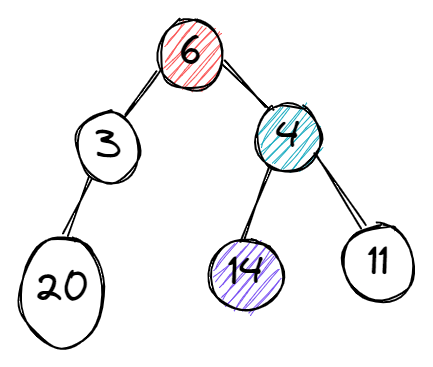
\includegraphics[width=0.3\linewidth]{Images/greedy.png}
    \caption{Thuật toán tham lam đi xác định điểm phù hợp gần nhất là điểm tối ưu}
    \label{fig:descGreedy}
\end{figure}

\subsubsubsection{Thuật toán sinh cột (Column Generation)}

\hspace{0.5cm}Sinh cột là một kỹ thuật phân rã mạnh mẽ, thường được sử dụng để giải các bài toán quy hoạch tuyến tính và tối ưu hóa tổ hợp quy mô lớn. Phương pháp này lặp đi lặp lại tinh chỉnh giải pháp bằng cách tạo ra các biến (cột) cải thiện hàm mục tiêu \cite{lubbecke2003columngeneration}.

\begin{itemize}
    \item \textbf{Cách hoạt động}: Phương pháp bắt đầu với một bài toán bị hạn chế chỉ bao gồm một tập hợp con của các biến. Một bài toán phụ định giá xác định các biến mới có tiềm năng nâng cao giải pháp. Các biến này được thêm vào lặp đi lặp lại cho đến khi không thể cải thiện thêm.
    \item \textbf{Ưu điểm}: Bằng cách tập trung vào một tập hợp con các biến tại mỗi lần lặp, sinh cột giúp giải quyết các bài toán với tập biến có kích thước lớn theo cấp số mũ.
    \item \textbf{Hạn chế}: Hiệu quả của sinh cột phụ thuộc vào việc giải quyết bài toán phụ định giá, điều này có thể trở nên khó khăn về mặt tính toán.
\end{itemize}

\begin{figure}[!htp]
    \centering
    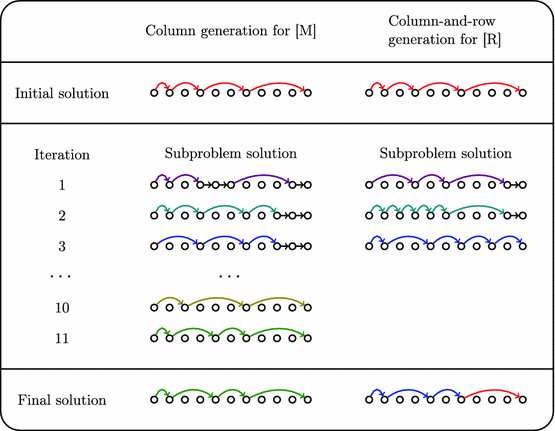
\includegraphics[width=0.35\linewidth]{Images/columngen.png}
    \caption{Quy trình sinh cột: Thêm biến lặp đi lặp lại}
    \label{fig:descColumnGen}
\end{figure}

\subsubsubsection{Thuật toán phân bổ tốt nhất (Best-Fit Algorithm)}
\hspace{0.5cm}Thuật toán phân bổ tốt nhất là một heuristic phổ biến trong việc giải quyết các bài toán đóng gói và phân bổ. Nó cố gắng tối thiểu hóa không gian lãng phí bằng cách đặt từng mục vào thùng hoặc ngăn phù hợp nhất \cite{cao2011bestfit}.

\begin{itemize}
    \item \textbf{Cách hoạt động}:
        \begin{itemize}
            \item Các mục được xử lý tuần tự.
            \item Mỗi mục được đặt vào thùng hoặc ngăn có không gian trống ít nhất mà vẫn đủ chứa mục.
            \item Nếu không tìm được thùng hoặc ngăn phù hợp, một thùng mới được mở.
        \end{itemize}
    \item \textbf{Ưu điểm}: Kỹ thuật này đơn giản và hiệu quả trong nhiều trường hợp thực tế.
    \item \textbf{Hạn chế}: Phương pháp có thể tạo ra các giải pháp kém tối ưu khi kích thước mục thay đổi hoặc các mục được xử lý không đồng nhất.
\end{itemize}




